% D10.1 Where the round-trip time goes (schematic, not to scale).
% Shared figure colours (colour only in figures).
\definecolor{robotfill}{HTML}{EAF2FC}\definecolor{robotline}{HTML}{2A78D6}
\definecolor{serverfill}{HTML}{FDEEE7}\definecolor{serverline}{HTML}{EB6834}
\definecolor{netfill}{HTML}{F0EFEC}\definecolor{greenfill}{HTML}{E9F5EC}\definecolor{greenline}{HTML}{2F9E58}
\definecolor{purplefill}{HTML}{F1ECF9}\definecolor{purpleline}{HTML}{7A55C7}
\definecolor{ink}{HTML}{0B0B0B}\definecolor{ink2}{HTML}{52514E}\definecolor{faultc}{HTML}{C9C6BF}

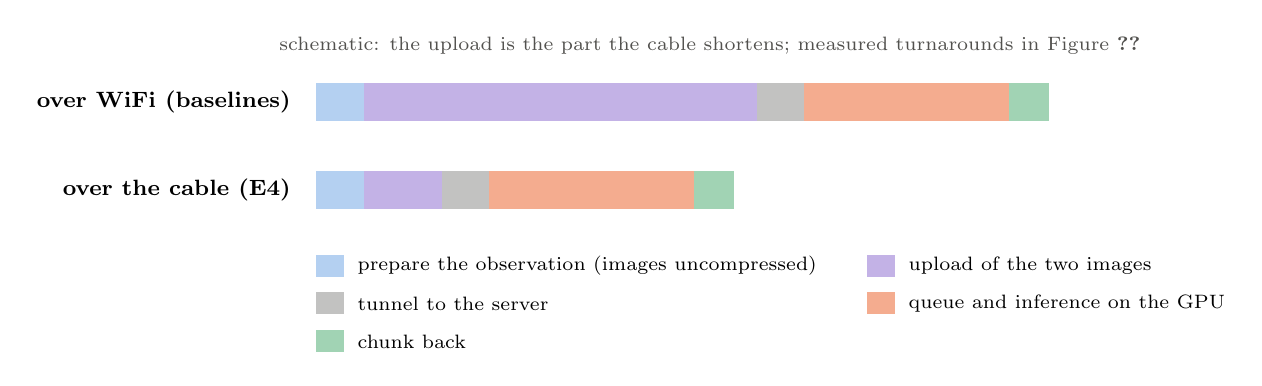
\begin{tikzpicture}[font=\footnotesize, x=10mm, y=8mm]
\foreach \y/\lab/\up in {1.4/{over WiFi (baselines)}/5.0, 0/{over the cable (E4)}/1.0} {
  \node[anchor=east, font=\footnotesize\bfseries] at (-0.2,\y) {\lab};
  \fill[robotline!35] (0,\y-0.3) rectangle ++(0.6,0.6);
  \fill[purpleline!45] (0.6,\y-0.3) rectangle ++(\up,0.6);
  \fill[ink2!35] (0.6+\up,\y-0.3) rectangle ++(0.6,0.6);
  \fill[serverline!55] (1.2+\up,\y-0.3) rectangle ++(2.6,0.6);
  \fill[greenline!45] (3.8+\up,\y-0.3) rectangle ++(0.5,0.6);}
\foreach \x/\y/\c/\t in {0/-1.2/robotline!35/{prepare the observation (images uncompressed)}, 7/-1.2/purpleline!45/{upload of the two images},
  0/-1.8/ink2!35/{tunnel to the server}, 7/-1.8/serverline!55/{queue and inference on the GPU}, 0/-2.4/greenline!45/{chunk back}} {
  \fill[\c] (\x,\y-0.17) rectangle ++(0.35,0.35); \node[anchor=west, font=\scriptsize] at (\x+0.4,\y) {\t};}
\node[font=\scriptsize, text=ink2] at (5,2.3) {schematic: the upload is the part the cable shortens; measured
  turnarounds in Figure~\ref{fig:edgertt}};
\end{tikzpicture}
